\documentclass[12pt]{amsart}
% packages
\usepackage{graphicx}
\usepackage{setspace}
\usepackage{amssymb,amsmath,amsthm,amsfonts,amscd}
\usepackage{hyperref}
\usepackage{color}
\usepackage{booktabs}
\usepackage{tabularx}
\usepackage{enumitem}
\usepackage[retainorgcmds]{IEEEtrantools}
\usepackage[notref,notcite,final]{showkeys}
\usepackage[final]{pdfpages}
\usepackage{fancyhdr}
\usepackage{upgreek}
\usepackage{multicol}
\usepackage{fontawesome}
\usepackage{halloweenmath}
\usepackage{ytableau}
% set margin as 0.75in
\usepackage[margin=0.75in]{geometry}

% tikz-related settings
\usepackage{tikz}
\usepackage{tikz-cd}
\usetikzlibrary{cd}

%% For table
\usepackage{tikz}
\usetikzlibrary{tikzmark}

% theorem environments with italic font
\newtheorem{thm}{Theorem}[section]
\newtheorem*{thm*}{Theorem}
\newtheorem{lemma}[thm]{Lemma}
\newtheorem{prop}[thm]{Proposition}
\newtheorem{claim}[thm]{Claim}
\newtheorem{corollary}[thm]{Corollary}
\newtheorem{conjecture}[thm]{Conjecture}
\newtheorem{question}[thm]{Question}
\newtheorem{procedure}[thm]{Procedure}
\newtheorem{assumption}[thm]{Assumption}

% theorem environments with roman font (use lower-case version in body
% of text, e.g., \begin{example} rather than \begin{Example})
\newtheorem{Definition}[thm]{Definition}
\newenvironment{definition}
{\begin{Definition}\rm}{\end{Definition}}
\newtheorem{Example}[thm]{Example}
\newenvironment{example}
{\begin{Example}\rm}{\end{Example}}

\theoremstyle{definition}
\newtheorem{remark}[thm]{\textbf{Remark}}

% special sets
\newcommand{\A}{\mathbb{A}}
\newcommand{\C}{\mathbb{C}}
\newcommand{\F}{\mathbb{F}}
\newcommand{\N}{\mathbb{N}}
\newcommand{\Q}{\mathbb{Q}}
\newcommand{\R}{\mathbb{R}}
\newcommand{\Z}{\mathbb{Z}}
\newcommand{\cals}{\mathcal{S}}
\newcommand{\ZZ}{\mathbb{Z}_{\ge 0}}
\newcommand{\cala}{\mathcal{A}}
\newcommand{\calb}{\mathcal{B}}
\newcommand{\cald}{\mathcal{D}}
\newcommand{\calh}{\mathcal{H}}
\newcommand{\call}{\mathcal{L}}
\newcommand{\calr}{\mathcal{R}}
\newcommand{\la}{\mathbf{a}}
\newcommand{\lgl}{\mathfrak{gl}}
\newcommand{\lsl}{\mathfrak{sl}}
\newcommand{\lieg}{\mathfrak{g}}

% math operators
\DeclareMathOperator{\kernel}{\mathrm{ker}}
\DeclareMathOperator{\image}{\mathrm{im}}
\DeclareMathOperator{\rad}{\mathrm{rad}}
\DeclareMathOperator{\id}{\mathrm{id}}
\DeclareMathOperator{\hum}{[\mathrm{Hum}]}
\DeclareMathOperator{\eh}{[\mathrm{EH}]}
\DeclareMathOperator{\lcm}{\mathrm{lcm}}
\DeclareMathOperator{\Aut}{\mathrm{Aut}}
\DeclareMathOperator{\Inn}{\mathrm{Inn}}
\DeclareMathOperator{\Out}{\mathrm{Out}}
\DeclareMathOperator{\Gal}{\mathrm{Gal}}


% frequently used shorthands
\newcommand{\ra}{\rightarrow}
\newcommand{\se}{\subseteq}
\newcommand{\ip}[1]{\langle#1\rangle}
\newcommand{\dual}{^*}
\newcommand{\inverse}{^{-1}}
\newcommand{\norm}[2]{\|#1\|_{#2}}
\newcommand{\abs}[1]{\lvert #1 \rvert}
\newcommand{\Abs}[1]{\bigg| #1 \bigg|}
\newcommand\bm[1]{\begin{bmatrix}#1\end{bmatrix}}
\newcommand{\op}{\text{op}}

% nicer looking empty set
\let\oldemptyset\emptyset
\let\emptyset\varnothing

%the var phi gang
\let\oldphi\phi
\let\phi\varphi

%\def\darktheme{} % IAN
\ifx \darktheme\undefined
\else
\pagecolor[rgb]{0.2,0.231,0.302}%{0.23,0.258,0.321}
\color[rgb]{1,1,1}
\fi

\def\multiset#1#2{\ensuremath{\left(\kern-.3em\left(\genfrac{}{}{0pt}{}{#1}{#2}\right)\kern-.3em\right)}}

\setlist[enumerate,1]{topsep=1em,leftmargin=1.8em, itemsep=0.5em, label=\textup{(}\arabic*\textup{)}}
\setlist[enumerate,2]{topsep=0.5em,leftmargin=3em, itemsep=0.3em}

%pagestyle
%\pagestyle{fancy} 

\begin{document}
\begin{center}
    \textsc{Math 502. HW 5\\ Ian Jorquera}
\end{center}
\vspace{1em}
% See http://www.mathematicalgemstones.com/maria/Math501Fall22.php
% for problems

% sage: https://sagecell.sagemath.org/
\begin{itemize}

\item[(1)] % % (2-) [3 points]
\iffalse
Sym=SymmetricFunctions(QQ)
s=Sym.schur()
m=Sym.monomial()
e=Sym.elementary()
h=Sym.homogeneous()
p=Sym.powersum()
s[3,1]*s[2,1]
\fi
Notice that $s_{3,1}\cdot s_{2,1}=s_{\rho/R}=\sum_\lambda c^{\rho}_{R\lambda}$ where $\rho=(5,4,3,1)$ and $R=(3,3)$. And so we must count the number of reverse ballot fillings of the skew tableau of shape $\rho/R$ which are shown below.

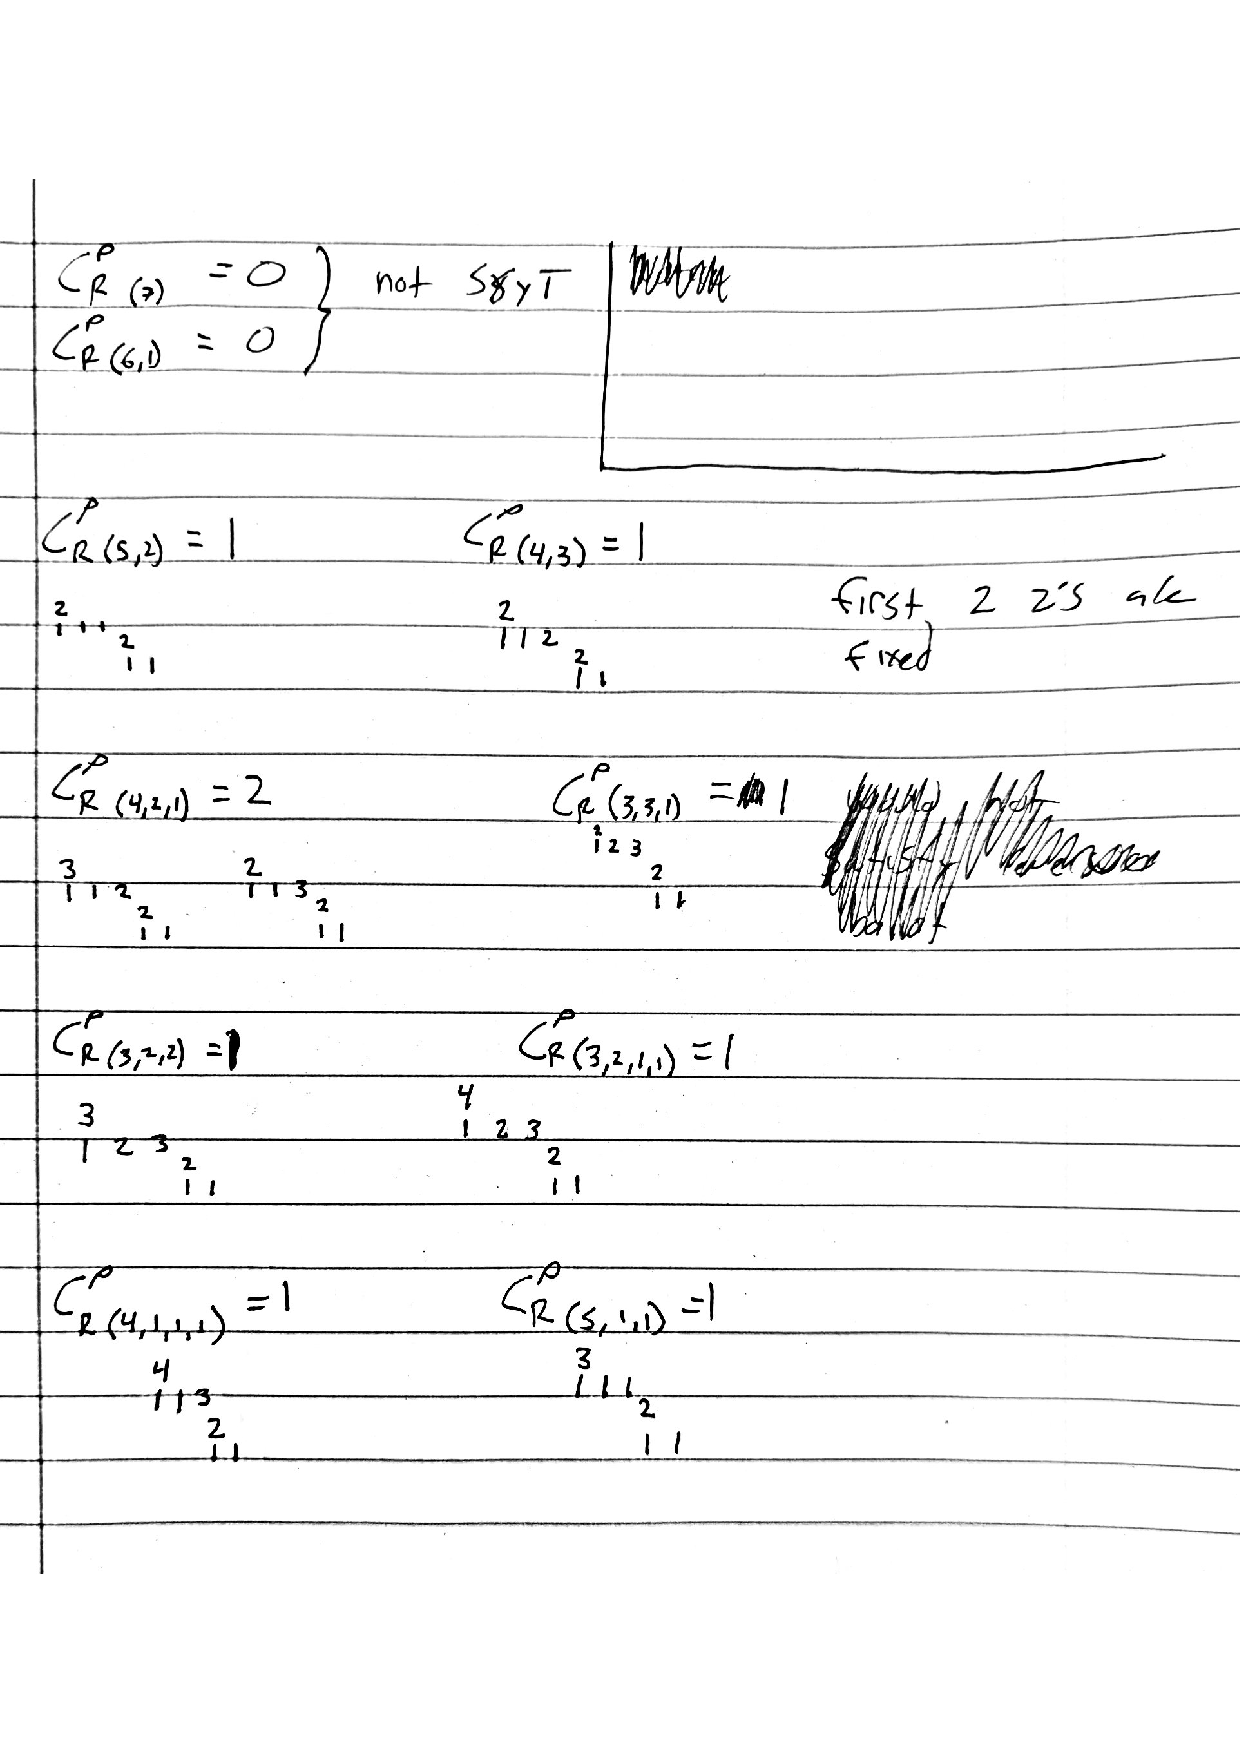
\includegraphics[scale=.6]{pics/hw6skew lr.pdf}

This give us $s_{3,1}\cdot s_{2,1}=s_{(5,2)}+s_{(4,3)}+2 s_{(4,2,1)}+s_{(3,3,1)}+s_{(3,2,2)}+s_{(3,2,1,1)}+s_{(4,1,1,1)}+s_{(5,1,1)}$.\\

\item[(4)] % (2) [3 points]
Consider the space orthogonal to the vector $(1)^n$ under the permutation representation where $\pi e_i = e_{\pi i}$ for any $\pi\in S_n$. This is the space $\text{span}(e_i-e_1 | 2\leq i\leq n)$. Notice that these are $n-1$ linearly independent vectors and so span the entire space orthogonal to $(1)^n$. notice also the for any $\pi\in S_n$ that $\pi(e_i-e_1)\cdot (1)^n=(e_{\pi i}-e_{\pi 1})\cdot (1)^n=(0)^n$, and so this subspace is a group representation. Now to see that this is isomorphic to $V_{(n-1,1)}=\text{span}((x_i-x_1)|2\leq i\leq n)$ notice that both spaces have the same dimension $n-1$ and so all we must show is that the group actions agree. Consider the linear map $\phi$ such that $\phi(x_i-x_1)=e_i-e_1$ and notice that $\phi(\pi(x_i-x_1))=\phi(x_{\pi i}-x_{\pi 1})=e_{\pi i}-e_{\pi 1}=\pi(e_i-e_1)=\pi\phi(x_i-x_1)$.\\

\item[(5)] % (2+) [4 points]  % Incomplete
Notice first the the regular representation is the vector space $V_r$ of formal sums of the elements of $S_3$ meaning it has order $6$. We will give an ordered basis $((),(1\;2),(1\;3),(2\;3),(1\;2\;3),(1\;3\;2))$ which we will use for constructing matrices. Furthermore because left multiplication by group elements defines a permutation of the group elements we know that each element $g\in S_3$ maps to a permutation matrix on the basis elements, the group elements. This means that the sum of all the group elements which corresponds to the matrix $(1)^6$ is Eigenvector with Eigenvalue $1$ for all each action. This corresponds to one of the irreducible factors being the trivial representation as every permutation fixes the vector. Notice that also the vector that assigns the odd permutations $-1$ and the even permutations $1$, or the vector $\begin{pmatrix}1&-1&-1&-1&1&1\end{pmatrix}^t$ under the ordered basis above, is also an eigenvector. This follows from the fact that multiplication by an odd permutation flips the sign of the permutation it is multiplied with and so has Eigenvalue $-1$. And multiplication by an even permutation preserves the sign of the permutation and so has Eigen Value $1$. This vector therefore corresponds to the sign permutation and the matrices result in a possible change of sign.\\

% Need more for this. Why is this the case. really just need to show no 1 dim vect space other then the two already found is preserved by group action
Finally notice that there are no other common eigenvectors for the matrices corresponding to the group actions of $S_3$. This means that there are no other $1$ dimensional irreducible representations and so there must be two copies of the standard representation which has dimension $2$.. And so $V_r=V_{(3)}\oplus V_{(1,1,1)}\oplus V_{(2,1)}\oplus V_{(2,1)}$.\\

We can also use characters. Notice that $\chi_{std}=(2\; 0\; -1)$, $\chi_{trv}=(1\; 1\; 1)$ and $\chi_{sgn}=(1\; -1\; 1)$ and because $\chi_{reg}=(6\; 0\; 0)$. Because the characters of a representation are a unique linear combination of the irreducibles we know that because $\chi_{reg}=\chi_{trv}+\chi_{sgn}+2\chi_{std}$, and so we know that $V_r=V_{(3)}\oplus V_{(1,1,1)}\oplus V_{(2,1)}\oplus V_{(2,1)}$.
\end{itemize}

\end{document}






